\chapter{Inleiding}
\label{chap:intro}

In deze template is de inleiding eerder een inleidend hoofdstuk in plaats van een inleiding in de pure betekenis van het woord. Daarom wordt dit hoofdstuk ook genummerd.

In Figuur~\ref{fig:cloud_rollen} wordt getoond...

\begin{figure}[h]
	\centering
	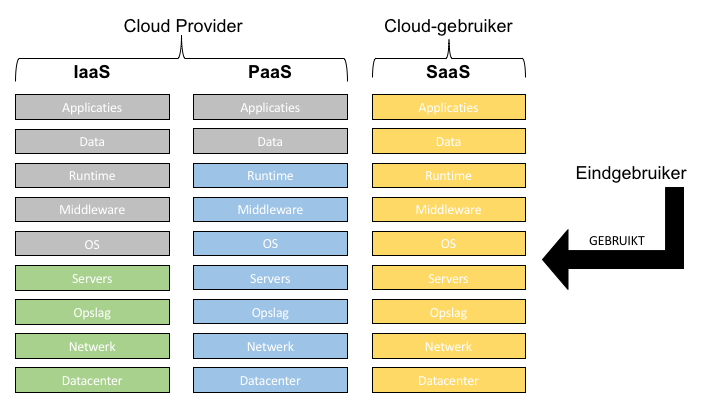
\includegraphics[width=\textwidth]{images/cloud_rollen.png}
	\caption{Image with caption.}
	\label{fig:cloud_rollen}
\end{figure}

Onderstaand codefragment ...

\begin{listing}[!h]
\begin{minted}[samepage]{js}
alert( 'Hello, world!' );
alert( 'Hello, world!' );
\end{minted}
\caption{Code embedded in document}
\end{listing}



\section{Sectie titel}

In Tabel~\ref{tab:resallocschemes} wordt een overzicht weergegeven ...

\begin{table}[h]
	\centering
	\captionsetup{justification=centering}
	\caption[Overzicht resource-allocatieschema's]{Overzicht resource-allocatieschema's}
	\label{tab:resallocschemes}
	\resizebox{\textwidth}{!}{%
	\begin{tabular}{L{4cm} l C{2cm} c c c c}
		\toprule
		Naam & Jaar & Type  & A | F | P  & Invoer & Uitvoer & Getest  \\ \midrule
		Alicherry et al.~\cite{Alicherry2012} & 2012 & k-sneden & A & G & par\{G\} & S \\
		MCRVMP~\cite{Biran2012} & 2012 & ILP \& GH & A & B\{netwerk\} & VM-plaatsing & C\\
		\bottomrule
	\end{tabular}}
\end{table}

In het volgende hoofdstuk~\ref{sec:related_work} wordt dieper ingegegaan op...
